\chapter{Преобразование алгебраических выражений}\label{chap:c09}\markright{Глава 11}
\begin{definition}\term{Подобные слагаемые} (\emph{like terms}) — слагаемые с одинаковой буквенной частью, включая показатели степеней.\end{definition}
\begin{definition}\term{Разложение на множители} (\emph{factorization}) — представление выражения в виде произведения.\end{definition}
\begin{definition}\term{Тождество} (\emph{identity}) — равенство, верное при всех допустимых значениях переменных.\end{definition}
\begin{definition}\term{Область допустимых значений (ОДЗ)} (\emph{admissible values; domain of an expression}) — значения переменных, при которых исходное выражение имеет смысл.\end{definition}
\section{Формулы сокращённого умножения}
\((a + b)^{2} = a^{2} + 2 ab + b^{2}\).\par
\((a - b)^{2} = a^{2} - 2 ab + b^{2}\).\par
\(a^{2} - b^{2} = (a - b) (a + b)\).\par
\section{Правила преобразований}
Общий множитель: \(ab + ac = a (b + c)\). Подобные слагаемые складывают по коэффициентам: \(2 x + 3 x = 5 x\).\par
В дроби сокращают общие множители числителя и знаменателя, а не отдельные слагаемые.\par
После сокращения сохраняют запреты исходного выражения. Знаменатель не равен \(0\); под квадратным корнем стоит неотрицательное число.\par
Чтобы убрать корень из знаменателя вида \(\sqrt{a} - b\), можно умножить числитель и знаменатель на \(\sqrt{a} + b\), если преобразование допустимо.\par
{\small\textit{Пример: \(\frac{x^{2} - 1}{x - 1} = x + 1\), но только при \(x \ne  1\).}}\par

\Needspace{7\baselineskip}\section*{Задачи}
\begingroup\setlength{\parskip}{2pt}
\noindent\begin{minipage}[t]{\linewidth}\textbf{11.1.} Раскрой скобки: \(3 (2 x - 5) - 2 (x + 1)\).\par\end{minipage}\par
\noindent\begin{minipage}[t]{\linewidth}\textbf{11.2.} Приведи подобные: \(4 a - 3 b + 2 a + 5 b\).\par\end{minipage}\par
\noindent\begin{minipage}[t]{\linewidth}\textbf{11.3.} Раскрой скобки: \((x + 3)^{2}\).\par\end{minipage}\par
\noindent\begin{minipage}[t]{\linewidth}\textbf{11.4.} Раскрой скобки: \((2 x - 1) (2 x + 1)\).\par\end{minipage}\par
\noindent\begin{minipage}[t]{\linewidth}\textbf{11.5.} Разложи на множители: \(6 x^{2} - 9 x\).\par\end{minipage}\par
\noindent\begin{minipage}[t]{\linewidth}\textbf{11.6.} Разложи на множители: \(x^{2} - 16\).\par\end{minipage}\par
\par\addvspace{5pt}\begin{lrbox}{\CatFlowBox}\begin{minipage}[t]{\linewidth}
\setlength{\parskip}{5pt}\setlength{\columnsep}{4.5mm}\setlength{\intextsep}{0pt}
\begin{wrapfigure}[12]{r}{54mm}

\includegraphics[width=54mm,height=58mm,keepaspectratio]{images/unique/art-16.png}
\label{catflow:16}
\end{wrapfigure}
\textbf{11.7.} Разложи на множители: \(x^{2} + 5 x + 6\).\par

\textbf{11.8.} Сократи \(\dfrac{x^{2} - 1}{x - 1}\). Укажи ограничения исходной дроби.\par

\textbf{11.9.} Упрости \(\dfrac{2}{x} + \dfrac{3}{2 x}\). Укажи ограничения.\par

\textbf{11.10.} Упрости \(\dfrac{a^{2} b}{ab^{2}}\). Укажи ограничения.\par

\textbf{11.11.} Упрости \(\dfrac{x^{2} - 4}{x^{2} + 4 x + 4}\). Укажи ограничения.\par

\textbf{11.12.} Упрости \(\dfrac{1}{\sqrt{5} - 2}\), избавившись от корня в знаменателе.\par

\textbf{11.13.} Билет стоит \(x\) рублей. Заказали \(3\) взрослых билета по полной цене и \(2\) детских по цене \(x - 100\) рублей. Составь и упрости выражение общей стоимости, если \(x > 100\).\par
\par\WFclear\end{minipage}\end{lrbox}%
\ifdim\dimexpr\ht\CatFlowBox+\dp\CatFlowBox\relax<64mm\dp\CatFlowBox=\dimexpr64mm-\ht\CatFlowBox\relax\fi%
\noindent\usebox{\CatFlowBox}\par\addvspace{5pt}

\noindent\begin{minipage}[t]{\linewidth}\textbf{11.14.} У прямоугольной клумбы стороны \(x + 2\) и \(x + 5\) метров, где \(x > 0\). Вырази площадь многочленом.\par\end{minipage}\par
\noindent\begin{minipage}[t]{\linewidth}\textbf{11.15.} Квадратную площадку со стороной \(x>0\) метров расширили на \(3\) м в каждом измерении. На сколько выросла её площадь?\begin{center}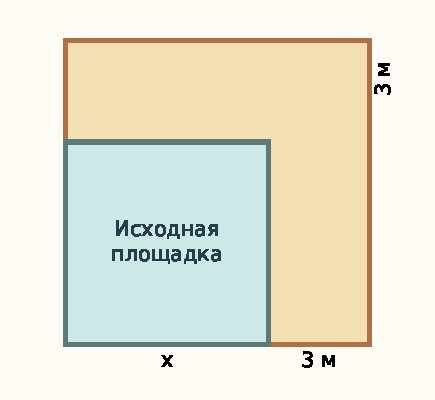
\includegraphics[width=.7\linewidth,height=45mm,keepaspectratio]{images/diagram-square.pdf}\end{center}\par\end{minipage}\par
\noindent\begin{minipage}[t]{\linewidth}\textbf{11.16.}\starmark{} Упрости \(\dfrac{x^{2} - 9}{x^{2} - x - 6}\) и укажи ОДЗ исходного выражения.\par\end{minipage}\par
\noindent\begin{minipage}[t]{\linewidth}\textbf{11.17.}\starmark{} Упрости: \((\dfrac{1}{x - 1} - \dfrac{1}{x + 1}) : (\dfrac{2}{x^{2} - 1})\).\par\end{minipage}\par
\noindent\begin{minipage}[t]{\linewidth}\textbf{11.18.}\starmark{} Докажи тождество \((a + b)^{2} - (a - b)^{2} = 4 ab\) и проверь его при \(a = 103,\allowbreak b = 97\), не вычисляя квадраты больших чисел.\par\end{minipage}\par
\noindent\begin{minipage}[t]{\linewidth}\textbf{11.19.} Докажите тождество \((a+b)^2+(a-b)^2=2a^2+2b^2\) для любых действительных \(a,b\).\par\end{minipage}\par
\noindent\begin{minipage}[t]{\linewidth}\textbf{11.20.} Докажите, что при \(x\neq-1\) и \(x\neq1\) выполнено \(\dfrac1{x-1}-\dfrac1{x+1}=\dfrac2{x^2-1}\). Объясните, зачем нужны оба исключения.\par\end{minipage}\par
\par\Needspace{12\baselineskip}\section*{Олимпиадные задачи}
\noindent\begin{minipage}[t]{\linewidth}\textbf{11.21.} {\small\itshape\href{https://mmo.mccme.ru/books/mmo-35-57.pdf}{ММО, 1940, I тур, 7–8 классы, № 1}; редакция условия.}\par Разложи на множители \((b-c)^3+(c-a)^3+(a-b)^3\).\par\end{minipage}\par
\noindent\begin{minipage}[t]{\linewidth}\textbf{11.22.} {\small\itshape\href{https://mmo.mccme.ru/books/mmo-35-57.pdf}{ММО, 1946, I тур, 7–8 классы, № 5}; редакция условия.}\par Докажи, что в произведении \((1-x+x^2-\cdots-x^{99}+x^{100})(1+x+x^2+\cdots+x^{100})\) коэффициенты всех нечётных степеней равны нулю.\par\end{minipage}\par
\endgroup
